
%https://tex.stackexchange.com/questions/25642/how-to-draw-a-line-of-dots-in-tikz

%https://tex.stackexchange.com/questions/45275/tikz-get-values-for-predefined-dash-patterns

% From:
% https://youtu.be/OCrO7jzavzA
% Channel: Master Your Academic Skills
% Video: latex tutorial: pgfplots tutorial: how to make a simple coordinate plot

%https://tex.stackexchange.com/questions/395287/tikz-for-loop-with-2-statements/395289

%\documentclass[border = 15 pt]{standalone}
%\documentclass[border = 10 pt]{standalone}
%\documentclass[border = 5 pt]{standalone}
\documentclass{standalone}

\standaloneconfig{border=.5mm .5mm .5mm .5mm}

%maths
\usepackage{mathtools}
\usepackage{amsmath}
\usepackage{amssymb}
\usepackage{amsfonts}

%tikzpicture
\usepackage{tikz}
\usepackage{scalerel}
\usepackage{pict2e}
\usepackage{tkz-euclide}
\usetikzlibrary{calc}
\usetikzlibrary{patterns, arrows.meta}
\usetikzlibrary{shadows}
\usetikzlibrary{external}

\usetikzlibrary{decorations.markings}

%pgfplots
\usepackage{pgfplots}
\pgfplotsset{compat=newest}
\usepgfplotslibrary{statistics}
\usepgfplotslibrary{fillbetween}

%colours
\usepackage{xcolor}

\newcommand*{\Scale}[2][4]{\scalebox{#1}{$#2$}}%%%%%

\usepackage{graphicx}

\usepackage{tikz-3dplot}

\usepackage{circuitikz}

\usetikzlibrary{shapes.geometric, arrows.meta, decorations.markings}

\pgfplotsset{compat = 1.17}

\tdplotsetmaincoords{60}{120}

\tikzset{
LM/.style = {very thin,
        {Bar[]Stealth}-%
        {Stealth[]Bar}
            },
% other common sty definitions like
every edge quotes/.append style= {font=\footnotesize}
        }

\tikzset{
LMT/.style = {thick,
        {Bar[]Stealth}-%
        {Stealth[]Bar}
            },
% other common sty definitions like
every edge quotes/.append style= {font=\footnotesize}
        }




\usepackage{xcolor}

\definecolor{groundElectron}{rgb}{0.0, 0.0, 0.55}
%\definecolor{groundElectron}{RGB}{140,140,140}

\definecolor{excitedElectron}{rgb}{1.0, 0.0, 0.22}
%\definecolor{excitedElectron}{RGB}{140,140,140}





\usetikzlibrary{decorations.pathreplacing,calligraphy}

\begin{document}

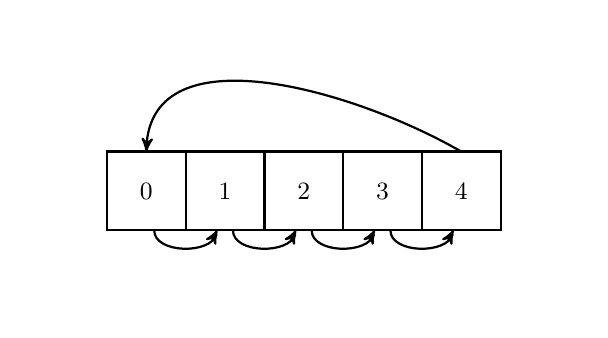
\begin{tikzpicture}

%%% Defining points:

\draw[white] (-1,-1) grid (6,2);

\coordinate (S1) at (0,0);
\coordinate (S2) at (1,0);
\coordinate (S3) at (2,0);
\coordinate (S4) at (3,0);
\coordinate (S5) at (4,0);

\coordinate (TX) at (1,0);
\coordinate (TY) at (0,1);

\draw[
     thick,
     black,
     ] 
     ($(S1)+0*(TX)+0*(TY)$) -- 
     ($(S1)+1*(TX)+0*(TY)$) -- 
     ($(S1)+1*(TX)+1*(TY)$) -- 
     ($(S1)+0*(TX)+1*(TY)$) -- 
     cycle;

\draw[
     thick,
     black,
     ] 
     ($(S2)+0*(TX)+0*(TY)$) -- 
     ($(S2)+1*(TX)+0*(TY)$) -- 
     ($(S2)+1*(TX)+1*(TY)$) -- 
     ($(S2)+0*(TX)+1*(TY)$) -- 
     cycle;

\draw[
     thick,
     black,
     ] 
     ($(S3)+0*(TX)+0*(TY)$) -- 
     ($(S3)+1*(TX)+0*(TY)$) -- 
     ($(S3)+1*(TX)+1*(TY)$) -- 
     ($(S3)+0*(TX)+1*(TY)$) -- 
     cycle;

\draw[
     thick,
     black,
     ] 
     ($(S4)+0*(TX)+0*(TY)$) -- 
     ($(S4)+1*(TX)+0*(TY)$) -- 
     ($(S4)+1*(TX)+1*(TY)$) -- 
     ($(S4)+0*(TX)+1*(TY)$) -- 
     cycle;

\draw[
     thick,
     black,
     ] 
     ($(S5)+0*(TX)+0*(TY)$) -- 
     ($(S5)+1*(TX)+0*(TY)$) -- 
     ($(S5)+1*(TX)+1*(TY)$) -- 
     ($(S5)+0*(TX)+1*(TY)$) -- 
     cycle;



\node[] at ($(S1)+0.5*(TX)+0.5*(TY)$) {\small{0}};
\node[] at ($(S2)+0.5*(TX)+0.5*(TY)$) {\small{1}};
\node[] at ($(S3)+0.5*(TX)+0.5*(TY)$) {\small{2}};
\node[] at ($(S4)+0.5*(TX)+0.5*(TY)$) {\small{3}};
\node[] at ($(S5)+0.5*(TX)+0.5*(TY)$) {\small{4}};




%\path[every node/.style={font=\sffamily\small}]
%    (S5) edge [bend right=90]  (S1);

\path[
	 thick,
	 black,
	 ->,
	 >=stealth',
	 main node/.style={circle,draw,font=\sffamily\Large\bfseries},
	 every node/.style={font=\sffamily\small},
	 ]
	 ($(S5)+0.5*(TX)+1*(TY)$) 
	 edge [out=150, in=90]  
	 ($(S1)+0.5*(TX)+1*(TY)$);

\path[
	 thick,
	 black,
	 ->,
	 >=stealth',
	 main node/.style={circle,draw,font=\sffamily\Large\bfseries},
	 every node/.style={font=\sffamily\small},
	 ]
	 ($(S1)+0.6*(TX)+0*(TY)$) 
	 edge [bend right=90]  
	 ($(S2)+0.4*(TX)+0*(TY)$);

\path[
	 thick,
	 black,
	 ->,
	 >=stealth',
	 main node/.style={circle,draw,font=\sffamily\Large\bfseries},
	 every node/.style={font=\sffamily\small},
	 ]
	 ($(S2)+0.6*(TX)+0*(TY)$) 
	 edge [bend right=90]  
	 ($(S3)+0.4*(TX)+0*(TY)$);

\path[
	 thick,
	 black,
	 ->,
	 >=stealth',
	 main node/.style={circle,draw,font=\sffamily\Large\bfseries},
	 every node/.style={font=\sffamily\small},
	 ]
	 ($(S3)+0.6*(TX)+0*(TY)$) 
	 edge [bend right=90]  
	 ($(S4)+0.4*(TX)+0*(TY)$);

\path[
	 thick,
	 black,
	 ->,
	 >=stealth',
	 main node/.style={circle,draw,font=\sffamily\Large\bfseries},
	 every node/.style={font=\sffamily\small},
	 ]
	 ($(S4)+0.6*(TX)+0*(TY)$) 
	 edge [bend right=90]  
	 ($(S5)+0.4*(TX)+0*(TY)$);

%https://tex.stackexchange.com/questions/228724/how-do-i-make-tikz-make-a-curved-arrow-from-one-node-to-another-when-my-nodes-ar/228726#228726




\end{tikzpicture}

\end{document}
